\chapter{Architecture du cœur MPTDC intégré dans SPADMIC}
\label{chap:architecture-mptdc}
\justifying
\sloppy

\section{Vue fonctionnelle}

Le cœur \textbf{MPTDC} transforme le principe Vernier multiphase étudié précédemment en une brique RTL intégrable dans la chaîne \textbf{SPADMIC}. L'architecture ne se limite pas à deux oscillateurs : elle associe la capture des événements \texttt{START}/\texttt{STOP}, la génération de phases lentes et rapides, une matrice de comparaison \mbox{$8\times8$}, une image de mesure figée, puis une lecture dans le domaine système. Les principaux paramètres architecturaux sont résumés dans le tableau \ref{tab:mptdc-params}.

\begin{table}[H]
    \centering
    \small
    \begin{tabular}{ll}
        \toprule
        \textbf{Paramètre} & \textbf{Valeur} \\
        \midrule
        Géométrie Vernier & $8 \times 8$ phases \\
        Pas de phase lent / rapide & \SI{55}{\pico\second} / \SI{50}{\pico\second} \\
        Différence élémentaire & \SI{5}{\pico\second} \\
        Pas brut de reconstruction & \SI{10}{\pico\second} \\
        Nombre de contextes & $2$ \\
        Détections exportables par conversion & jusqu'à $15$ \\
        Horloge système & \SI{160}{\mega\hertz} \\
        Interface de sortie & trame compacte sur bus \SI{16}{\bit} \\
        \bottomrule
    \end{tabular}
    \caption{Paramètres architecturaux principaux de l'implémentation \textbf{MPTDC}.}
    \label{tab:mptdc-params}
\end{table}

\begin{figure}[H]
    \centering
    
\includegraphics[width=\textwidth]{tdc/mptdc_block_diagram.pdf}
    \caption{Vue fonctionnelle du cœur MPTDC. Les événements arment les oscillateurs ; les faisceaux de phases alimentent la matrice Vernier ; le domaine système récupère ensuite des compteurs synchronisés, une image de mesure figée et un flux de lecture compact.}
    \label{fig:mptdc-block-diagram}
\end{figure}

La figure \ref{fig:mptdc-block-diagram} met en évidence la séparation des responsabilités. Les phases lentes et rapides restent locales aux oscillateurs et à la matrice ; elles ne deviennent pas un bus synchrone continu dans \texttt{clk\_sys}. Le domaine système reçoit seulement des informations stabilisées : compteurs Gray synchronisés, commandes de capture, image de contexte et flux de lecture. C'est cette séparation qui rend le bloc à la fois mesurable et intégrable.

\begin{table}[H]
    \centering
    \scriptsize
    \begin{tabularx}{\textwidth}{>{\raggedright\arraybackslash}p{4.0cm}>{\raggedright\arraybackslash}p{2.4cm}>{\raggedright\arraybackslash}X}
        \toprule
        \textbf{Fonction matérielle} & \textbf{Domaine} & \textbf{Rôle} \\
        \midrule
        Interface de capture asynchrone & Asynchrone & Mémorisation de \texttt{START}/\texttt{STOP}, acceptation de la conversion et démarrage des anneaux \\
        \midrule
        Générateurs de phases lent et rapide & Oscillateurs & Production locale des huit sorties de phase utilisées par la comparaison Vernier \\
        \midrule
        Compteurs grossiers Gray & Lent / rapide & Comptage large et transfert sécurisé vers le domaine système \\
        \midrule
        Matrice de phase & Rapide & Détection des croisements entre phases lentes et rapides \\
        \midrule
        Capture de métadonnées temporelles & Asynchrone & Conservation d'informations auxiliaires utiles aux cas de frontière \\
        \midrule
        Banque de contextes & Image figée & Conservation atomique d'une conversion terminée \\
        \midrule
        Lecture et sérialisation & \texttt{clk\_sys} & Lecture du contexte, file FIFO et émission de la trame \SI{16}{\bit} \\
        \midrule
        Surveillance & Mixte & Fermeture contrôlée en cas d'événement manquant, de blocage ou de timeout \\
        \bottomrule
    \end{tabularx}
    \caption{Répartition fonctionnelle des principales briques matérielles. Les noms exacts des modules RTL restent propres à l'implémentation ; la description conserve ici une lecture système.}
    \label{tab:mptdc-module-map}
\end{table}

\section{Capture et cœur Vernier}

La capture de \texttt{START}/\texttt{STOP} reste volontairement asynchrone. Un échantillonnage préalable par \texttt{clk\_sys} simplifierait le RTL, mais il déplacerait l'incertitude temporelle sur le chemin même que le TDC cherche à mesurer. Le choix retenu consiste donc à déclencher directement l'anneau lent au front \texttt{START}, puis l'anneau rapide au front \texttt{STOP}. Le chronogramme de la figure \ref{fig:async-capture-timing}, introduit au chapitre précédent, résume cette logique par deux latches \textit{set/reset} et un nettoyage ultérieur par le domaine système.

Une fois les deux anneaux actifs, la matrice \mbox{$8\times8$} compare les huit sorties de phase lentes aux huit sorties de phase rapides. Chaque cellule mémorise le passage utile et fournit une information fine locale. En parallèle, les compteurs grossiers donnent la position large de la conversion. L'architecture exporte aussi des métadonnées de contexte et de frontière ; elles ne sont pas destinées à être interprétées bit par bit dans cette description fonctionnelle, mais elles rendent observables les cas ambigus au voisinage des transitions lentes.

Ce point explique un compromis central. La grille fine issue de la matrice n'est pas uniformément remplie : certains codes sont absents ou moins denses. Le bloc ne tente pas de corriger cette non-uniformité dans le silicium. Il exporte plutôt une image de mesure suffisamment riche pour que la calibration externe reconstruise ensuite un temps corrigé.

\section{Protocole de mesure, gel de l'image et réarmement}

La fin d'une conversion n'est pas simplement un ordre de lecture. Elle forme un court protocole de mesure qui protège l'information temporelle avant toute remise à zéro de la matrice. La séquence peut se lire en cinq étapes : \texttt{START} lance l'anneau lent ; \texttt{STOP} lance l'anneau rapide et ouvre la fenêtre de détection ; la matrice mémorise les croisements utiles ; la logique système fige une image cohérente de la conversion ; puis elle nettoie la fenêtre de mesure pour rendre le bloc disponible à l'événement suivant.

La figure \ref{fig:timing-diagram-conversion} explicite cette transition entre le domaine Vernier et le domaine système. La fenêtre de détection active la matrice de phase. Lorsqu'au moins une cellule a mémorisé un croisement et que la conversion est complète, la logique de contrôle déclenche d'abord le gel de l'image, puis l'écriture dans la banque de contextes. Le nettoyage intervient seulement après cette protection : il réarme la matrice sans détruire la conversion déjà capturée.

Les noms internes ne sont utiles ici que comme repères : la fenêtre de détection (\texttt{pd\_gate}) autorise les cellules de la matrice ; le niveau de détection (\texttt{hit\_level}) indique qu'un croisement a été mémorisé ; l'état de mesure complète (\texttt{meas\_active}) demande la prise en charge par le domaine système ; puis \texttt{snapshot\_en}, \texttt{capture\_en} et \texttt{clear} figent, écrivent et nettoient la conversion.

\begin{figure}[H]
    \centering
    
\includegraphics[width=\textwidth]{tdc/timing_diagram_conversion.pdf}
    \caption{Protocole de fermeture d'une mesure. La FSM système observe la fin de conversion, fige l'image de la matrice, écrit le contexte, nettoie la fenêtre de détection puis autorise la lecture.}
    \label{fig:timing-diagram-conversion}
\end{figure}

Le snapshot protège donc les données avant tout nettoyage, ce qui évite de perdre l'image de mesure pendant que la chaîne de lecture travaille à un rythme plus lent.

Il faut distinguer ce protocole de mesure du protocole de lecture. Le premier a pour rôle de produire une image atomique et stable ; le second parcourt ensuite le contexte figé, construit les enregistrements, les amortit par une file FIFO synchrone et les transmet vers la sortie \SI{16}{\bit}. Le format maintenu reste volontairement compact : un en-tête, deux mots par enregistrement de détection, nommé \texttt{HIT} dans le protocole RTL, et un mot de fin de conversion,
\[
    N_{\mathrm{mots}} = 2\,N_{\mathrm{det}} + 2.
\]
Chaque ligne de la trame correspond à un mot de \SI{16}{\bit}. Les bits hauts identifient la classe du mot, tandis que la charge utile transporte soit le contexte de conversion, soit les composantes de l'enregistrement de détection, soit l'information de fin de paquet. Les positions de bits sont celles du protocole maintenu ; les informations auxiliaires de calibration sont regroupées sous des champs de statut ou de métadonnées afin de conserver une lecture système.

\begin{figure}[H]
    \centering
    \small
    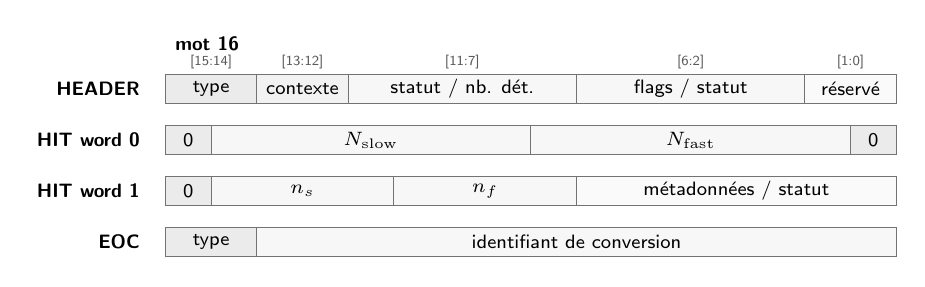
\begin{tikzpicture}[
        x=0.58cm,
        y=0.72cm,
        champ/.style={draw=black!55,line width=0.45pt,align=center,font=\sffamily\scriptsize},
        nom/.style={anchor=east,font=\sffamily\scriptsize\bfseries},
        plage/.style={font=\sffamily\tiny,text=black!65}
    ]
        \node[anchor=west,font=\sffamily\scriptsize\bfseries] at (0,4.05) {mot \SI{16}{\bit}};
        \node[plage] at (1,3.72) {[15:14]};
        \node[plage] at (3,3.72) {[13:12]};
        \node[plage] at (6.5,3.72) {[11:7]};
        \node[plage] at (11.5,3.72) {[6:2]};
        \node[plage] at (15,3.72) {[1:0]};

        \node[nom] at (-0.35,3.25) {HEADER};
        \draw[champ,fill=black!8] (0,3.0) rectangle (2,3.5); \node[champ,draw=none] at (1,3.25) {type};
        \draw[champ,fill=black!5] (2,3.0) rectangle (4,3.5); \node[champ,draw=none] at (3,3.25) {contexte};
        \draw[champ,fill=black!3] (4,3.0) rectangle (9,3.5); \node[champ,draw=none] at (6.5,3.25) {statut / nb. dét.};
        \draw[champ,fill=black!3] (9,3.0) rectangle (14,3.5); \node[champ,draw=none] at (11.5,3.25) {flags / statut};
        \draw[champ,fill=black!2] (14,3.0) rectangle (16,3.5); \node[champ,draw=none] at (15,3.25) {réservé};

        \node[nom] at (-0.35,2.35) {HIT word 0};
        \draw[champ,fill=black!8] (0,2.1) rectangle (1,2.6); \node[champ,draw=none] at (0.5,2.35) {0};
        \draw[champ,fill=black!3] (1,2.1) rectangle (8,2.6); \node[champ,draw=none] at (4.5,2.35) {$N_{\mathrm{slow}}$};
        \draw[champ,fill=black!3] (8,2.1) rectangle (15,2.6); \node[champ,draw=none] at (11.5,2.35) {$N_{\mathrm{fast}}$};
        \draw[champ,fill=black!8] (15,2.1) rectangle (16,2.6); \node[champ,draw=none] at (15.5,2.35) {0};

        \node[nom] at (-0.35,1.45) {HIT word 1};
        \draw[champ,fill=black!8] (0,1.2) rectangle (1,1.7); \node[champ,draw=none] at (0.5,1.45) {0};
        \draw[champ,fill=black!3] (1,1.2) rectangle (5,1.7); \node[champ,draw=none] at (3,1.45) {$n_s$};
        \draw[champ,fill=black!3] (5,1.2) rectangle (9,1.7); \node[champ,draw=none] at (7,1.45) {$n_f$};
        \draw[champ,fill=black!2] (9,1.2) rectangle (16,1.7); \node[champ,draw=none] at (12.5,1.45) {métadonnées / statut};

        \node[nom] at (-0.35,0.55) {EOC};
        \draw[champ,fill=black!8] (0,0.3) rectangle (2,0.8); \node[champ,draw=none] at (1,0.55) {type};
        \draw[champ,fill=black!3] (2,0.3) rectangle (16,0.8); \node[champ,draw=none] at (9,0.55) {identifiant de conversion};
    \end{tikzpicture}
    \caption{Schéma synthétique du format de sortie \SI{16}{\bit}. Le paquet commence par un en-tête, encode chaque enregistrement de détection sur deux mots \texttt{HIT}, puis se termine par un mot de fin de conversion. Les champs de métadonnées regroupent les informations auxiliaires nécessaires au décodage et à la calibration externe, sans détailler ici les signaux RTL internes.}
    \label{fig:mptdc-output-frame}
\end{figure}
Les informations auxiliaires de calibration sont intégrées à cette trame sans introduire de mode de sortie concurrent. Le réarmement est ainsi amélioré : dès qu'une conversion est protégée dans un contexte, le cœur peut préparer une nouvelle fenêtre de mesure sans attendre que tout le paquet précédent soit transmis. Si la lecture aval est suspendue, le parcours du contexte conserve sa position ; si les deux contextes restent occupés trop longtemps, le bloc rend cette situation observable par ses champs de statut.

\clearpage

\section{Extraits RTL représentatifs des choix d'architecture}

Les extraits suivants ne recopient pas des modules complets. Ils isolent deux décisions d'architecture présentes dans le RTL actif : la protection de l'image de mesure avant nettoyage, puis le transfert de compteurs par code Gray et synchronisation. Les exemples sont volontairement courts ; ils montrent le contrat matériel retenu plutôt que tous les détails de typage, de reset ou d'observabilité.

\begin{rtlSnippet}{Extrait simplifié fidèle : snapshot avant clear}
unique case (state_q)
  ST_M_IDLE:     if (meas_active_i) state_d = ST_M_MEASURE;
  ST_M_MEASURE:  state_d = ST_M_SNAPSHOT;
  ST_M_SNAPSHOT: state_d = ST_M_COUNT;
  ST_M_COUNT:    state_d = ST_M_EVAL;
  ST_M_EVAL:     state_d = ST_M_CAPTURE;
  ST_M_CAPTURE:  state_d = ST_M_CLEAR;
  ST_M_CLEAR:    state_d = ST_M_IDLE;
endcase

assign snapshot_en_o = (state_q == ST_M_SNAPSHOT);
assign capture_en_o  = (state_q == ST_M_CAPTURE);
assign fe_clear_o    = (state_q == ST_M_CAPTURE);
assign pd_clear_o    = (state_q == ST_M_CLEAR);
\end{rtlSnippet}

Le choix retenu protège l'image de mesure avant toute remise à zéro de la matrice. L'état \texttt{SNAPSHOT} échantillonne le bus statique de détections et de tags ; les états \texttt{COUNT} et \texttt{EVAL} découpent la réduction des détections et l'évaluation des flags ; l'état \texttt{CAPTURE} écrit le contexte et libère le front-end ; l'état \texttt{CLEAR} nettoie ensuite la matrice source. L'effet PPA attendu est une réduction du temps mort côté capture, car le front-end n'attend pas la fin de la sérialisation. Le coût est une image de contexte supplémentaire et quelques cycles \texttt{clk\_sys}. Le goulot se déplace vers l'occupation des deux contextes sous rétropression aval ; il est traité par les statuts d'occupation, le rejet contrôlé de nouveaux \texttt{START} et la libération explicite du contexte par le drain.

\begin{rtlSnippet}{Extrait simplifié fidèle : compteur Gray synchronisé}
always_ff @(posedge src_clk or negedge src_rst_n or posedge src_async_clr) begin
  if (!src_rst_n || src_async_clr) begin
    gray_src_cont_q      <= '0;
    gray_src_snap_sync_q <= '0;
  end else begin
    // Un seul bit change entre deux valeurs Gray adjacentes.
    gray_src_cont_q      <= gray_encode_value ^ (gray_encode_value >> 1);
    gray_src_snap_sync_q <= bin_snap_q ^ (bin_snap_q >> 1);
  end
end

assign gray_src_snap_sel = USE_ASYNC_SNAPSHOT ? gray_src_snap_async_q
                                              : gray_src_snap_sync_q;

always_ff @(posedge dst_clk or negedge dst_rst_n) begin
  if (!dst_rst_n) begin
    gray_cont_ff1_async <= '0;
    gray_cont_ff2_async <= '0;
    gray_snap_ff1_async <= '0;
    gray_snap_ff2_async <= '0;
  end else begin
    gray_cont_ff1_async <= gray_src_cont_q;
    gray_cont_ff2_async <= gray_cont_ff1_async;
    gray_snap_ff1_async <= gray_src_snap_sel;
    gray_snap_ff2_async <= gray_snap_ff1_async;
  end
end
\end{rtlSnippet}

Le deuxième extrait montre le principe utilisé pour les compteurs grossiers : la valeur source est convertie en Gray, puis traversée par une chaîne de synchronisation dans le domaine de destination. Le choix RTL réduit le risque d'image incohérente lors du passage entre domaines, car une transition Gray ne modifie qu'un bit logique à la fois. L'impact PPA est le coût de quelques bascules de synchronisation et d'une conversion Gray/binaire, très inférieur au risque d'un bus binaire multi-bit directement échantillonné. Le goulot déplacé est la latence de synchronisation, acceptable ici car les compteurs servent à reconstruire une image de mesure déjà figée, et non à piloter en temps réel les phases rapides.

\section{Robustesse et vérification}

La robustesse repose sur plusieurs niveaux complémentaires. Une surveillance lente ferme les conversions dont le \texttt{STOP} n'arrive pas, une surveillance de mesure évite qu'une fenêtre reste active trop longtemps, et une surveillance système protège le bloc contre les absences globales de progression. Dans le RTL actuel, les fenêtres de surveillance sont exposées par les registres de contrôle lents : le timeout par contexte et le timeout global sont programmables sur \SI{16}{\bit}. Une valeur non nulle fixe le seuil utilisé ; une valeur nulle sélectionne le repli interne de \num{64} cycles \texttt{clk\_sys} pour la fermeture \texttt{START} sans \texttt{STOP}, tandis qu'elle désactive la surveillance globale. Les champs de statut rendent ensuite observable une fermeture par watchdog ou une absence globale de progression. Ces mécanismes ne remplacent pas la validation physique finale, mais ils rendent le RTL testable et récupérable dans les scénarios de blocage.

La vérification a été conduite avec une méthodologie proche de l'industrie, sans dépendre d'un seul banc monolithique. Des bancs unitaires vérifient les briques isolées ; des bancs d'intégration vérifient les chemins complets de conversion ; des scénarios dirigés et aléatoires explorent les cas nominaux et limites ; un modèle de référence permet de comparer systématiquement les paquets attendus aux paquets observés. Les points vérifiés couvrent notamment la cohérence de la trame, la rétropression, les resets, les timeouts, les rejets d'événements et les transitions proches des frontières de mesure.

Cette validation reste une validation RTL. Elle donne une confiance forte dans le comportement fonctionnel, dans l'ordre de lecture et dans le contrat de paquetisation, mais elle ne remplace ni la revue CDC complète, ni la STA, ni la simulation post-layout avec les oscillateurs réels.

\section{Lien avec la caractérisation}

L'architecture est conçue pour déplacer la correction temporelle hors ASIC. Le silicium exporte une description stable de la conversion ; le décodeur hôte et la LUT de calibration transforment ensuite ces observables en temps corrigé. Le chapitre \ref{chap:resultats-calibration} se concentre donc sur la question quantitative : les informations exportées suffisent-elles à corriger la non-uniformité du codage brut dans une campagne RTL/Xcelium tenue hors apprentissage ?

\begin{summaryBox}
Le cœur \textbf{MPTDC} réalise le compromis attendu pour \textbf{SPADMIC} : capture asynchrone au plus près des événements, matrice Vernier compacte, image de mesure protégée, double contexte, lecture \texttt{clk\_sys} et trame \SI{16}{\bit}. Les détails RTL fins restent subordonnés au contrat système et aux choix qui conditionnent la caractérisation.
\end{summaryBox}

\clearpage
